\documentclass[compress]{beamer}
\usepackage{fontspec,fontawesome,tikz}

\usetheme{Nord}
\setmainfont{Yanone Kaffeesatz}
\setsansfont{Roboto Condensed}
\setmonofont[Scale=0.85]{Inconsolata}
\newfontfamily\segoefont[]{Segoe Print}
\newfontfamily\stmfont{Share Tech Mono}


\title{SciPy v1.5.1}
\subtitle{Brief update + some pep-talk}
\author{\.Ilhan Polat}
\date{08/07/2020}

\begin{document}

\begin{frame}[plain,noframenumbering]
  \maketitle
\begin{tikzpicture}[remember picture,overlay]
\node[rotate=55,NordWhite] (dolores) at ([shift={(-2.8cm,2.8cm)}]current page.center) {\segoefont meters};
\begin{scope}[shift={([shift={(-7mm,-10mm)}]dolores.south)}]
    \draw[line cap=round,ultra thick, NordWhite,overlay] (0,0) -- ++(1mm,1mm) -- ++(0.75mm,-0.75mm);
\end{scope}
\end{tikzpicture}
\end{frame}

\begin{frame}[fragile]{About me}
\begin{description}[Snow Storm]
\item[SciPy] Member for \textasciitilde 3 years
\item[based] Amsterdam, NL
\item[works @] \tikz[baseline={([yshift=-.5ex]current bounding box.center)}]{\node[scale=0.3,rounded corners,draw=white,fill=white]{
\includegraphics[]{edlogotrimmed}};}
\item[day-job] IoT, Predictive Maintenance, Condition Monitoring
\item[ex-academia] Control Theory, check out \textcolor{NordYellow}{\stmfont harold} on GitHub
\item[social] \begin{tabular}{cl}\faGithubSquare&@ilayn\\\faLinkedinSquare&ilhanpolat\\\faTwitterSquare&\_ilhanpolat\_\\\faEnvelopeSquare&ilhanpolat@gmail.com\end{tabular}
\end{description}
\end{frame}

\begin{frame}{SciPy Updates}{v1.5.1}
\begin{description}[Snow Storm]
\item[\faUsers] 129 people contributed.
\item[\faBug] 168 issues closed.
\item[\faMedkit] 471 pull requests merged.
\end{description}

\vspace{1cm}

\hspace{1cm}5 minute rule $\to$ \textasciitilde25 mins/contributor
\end{frame}

\begin{frame}[fragile]{SciPy Updates}{{\stmfont linalg}}
\begin{description}[Snow Storm]
\item[scipy.linalg.eigh] New facelift and subset of eigs based on index or value.
\item[scipy.linalg.lapack] Lots of new low-level LAPACK wrappers (more to come).
\item[scipy.linalg.cossin] Cosine-Sine Decomposition of unitary matrices.
\end{description}
\end{frame}

\begin{frame}[fragile]{SciPy Updates}{{\stmfont stats}}
\begin{description}[Snow Storm]
\item[Performance] speed for many and accuracy for some
\item[Random Seeds] Support for newer {\stmfont np.random.Generator}
\item[Kolmogorov-Smirnov] 2-sided 1-sample added, now handles 1-sample and 2-sample tests
\end{description}
\end{frame}

\begin{frame}[fragile]{SciPy Updates}{{\stmfont optimize}}
\begin{description}[Snow Storm]
\item[scipy.optimize.linprog] presolve and constraint handler are faster.
\item[scipy.optimize.minimize] Absolute and relative step size enhancements + simple caching.
\end{description}
\end{frame}

\begin{frame}[fragile]{SciPy Updates}{Other Modules}
\begin{block}{Too many to enumerate}
	\textcolor{NordWhite}{Check out the release notes for more:}
    
    \textcolor{NordYellow}{\stmfont\small https://github.com/scipy/scipy/releases/tag/v1.5.0}
\end{block}
\end{frame}

\begin{frame}[fragile]{SciPy Team}{Status}
\begin{description}[Snow Storm]
\item[Total] 61 members
\item[Active] >23 members
\item[Open] 1234 Issues, 291 PRs
\end{description}

\begin{tikzpicture}[remember picture, overlay]
\node[NordWhite,font=\tiny,text opacity=0.5] at ([shift={(3cm,1.1cm)}]current page.center) {
\begin{tabular}{lll}
Atsushi Sakai       &Ilhan Polat     &Nikolay Mayorov   \\
Andrew Nelson       &Josef Perktold  &Paul van Mulbregt \\
Christoph Baumgarten&Josh Wilson     &Pauli Virtanen    \\
CJ Carey            &Kai Striega     &Peter Bell        \\
Eric Larson         &Lucas Roberts   &Peter Larsen      \\
Evgeni Burovski     &Matt Haberland  &Ralf Gommers      \\
Gregory R. Lee      &Matthew Brett   &Seth Troisi       \\
Tyler Reddy         &Warren Weckesser&
\end{tabular}};
\end{tikzpicture}

\vspace{1cm}

\hspace{1cm}5 minute rule $\to$ \textasciitilde 6.5 hours/active maintainer

\end{frame}

\begin{frame}{Maintaining SciPy}{Personal}
\begin{itemize}
\item Socially demanding
\item Requires some personal introspection
\item Depends on package-specific past experience
\end{itemize}
\end{frame}

\begin{frame}{Maintaining SciPy}{Personal}
  \begin{columns}[T]
    \begin{column}[t]{0.5\textwidth} 
    {
      \centering 
      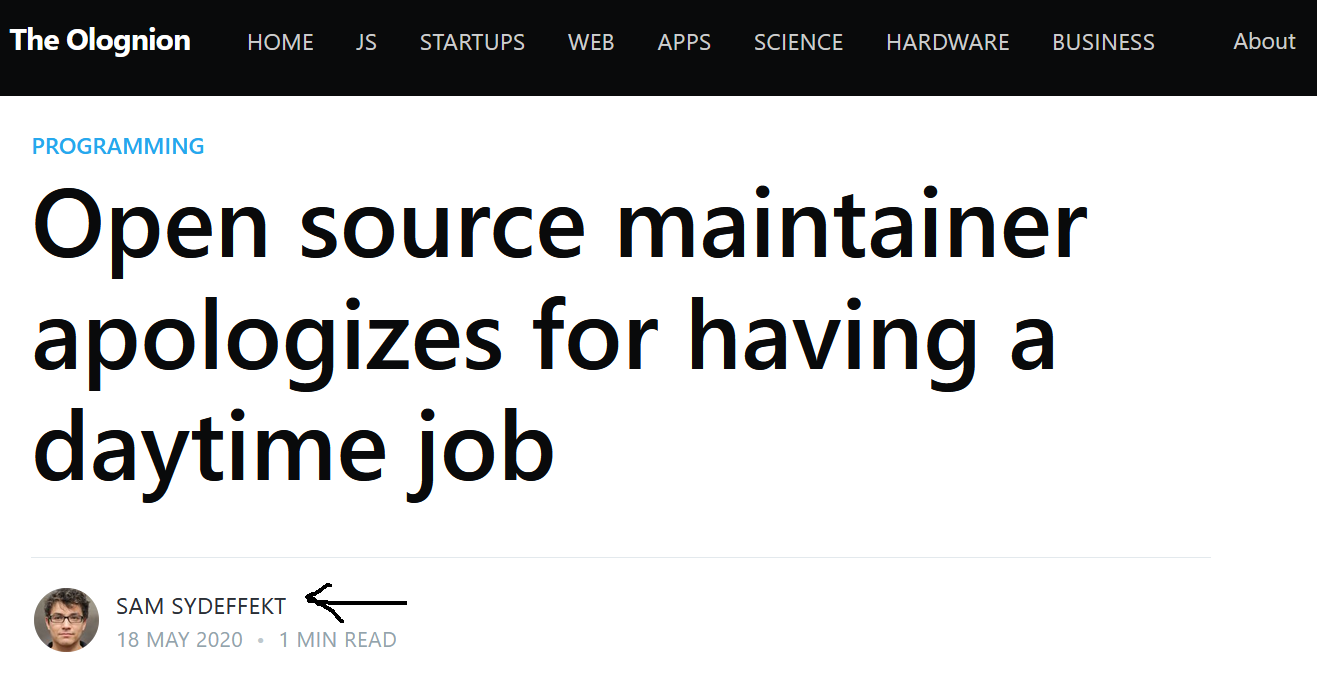
\includegraphics[width=0.8\textwidth]{olognion}
      \par
    }
    \vspace{1cm}
    \visible<3>{
        \centering 
        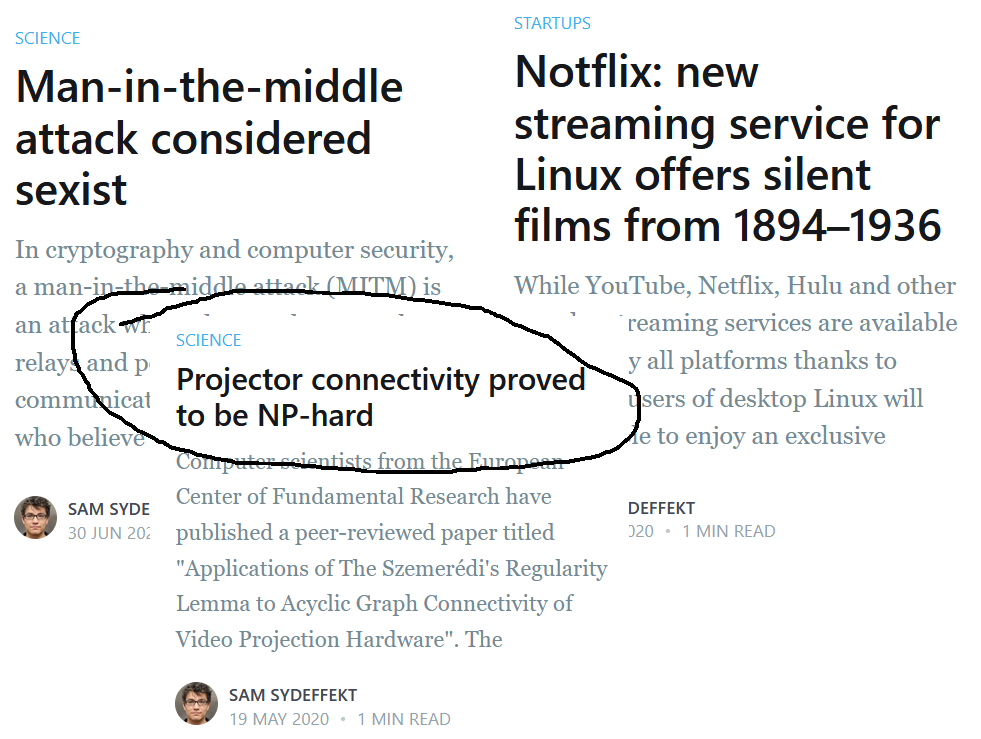
\includegraphics[width=0.8\textwidth]{nuggets}
        \par
        {\stmfont\tiny https://www.theolognion.com/}
    }
    \end{column}
    \begin{column}[c]{0.55\textwidth}
    \visible<2->{
        \centering 
        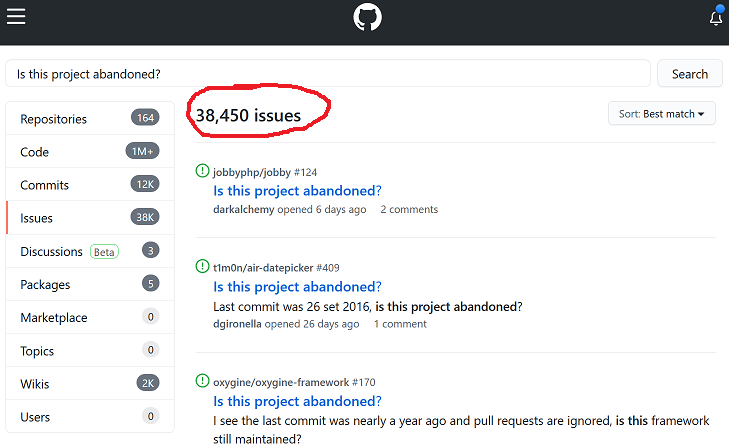
\includegraphics[width=0.8\textwidth]{abandon}
        \par
        {\stmfont\tiny https://opensource.com/article/20/5/adoptoposs}
    }
   \end{column}
  \end{columns}
\end{frame}

\begin{frame}{Maintaining SciPy}{Legacy}
{
\centering 
\begin{tikzpicture}
\node[inner sep=0] (a) {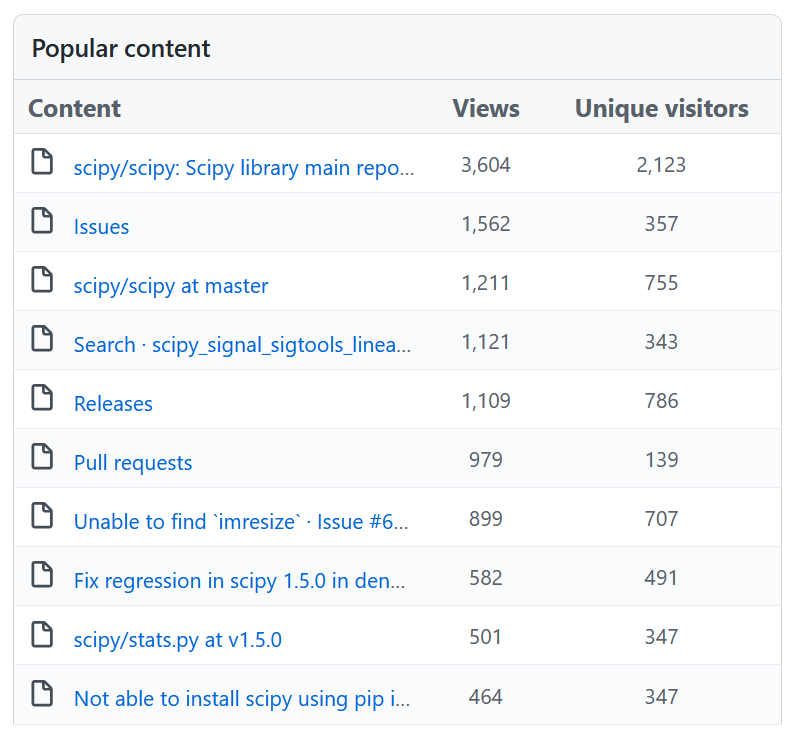
\includegraphics[scale=0.5]{imresize}};
\draw<2->[black, ultra thick][rounded corners](a.-155) rectangle (a.-15);
\end{tikzpicture}
\par
}
\end{frame}

\begin{frame}{Maintaining SciPy}{Responsibility}
{
\centering 

\includegraphics[width=0.9\textwidth]{pinv1}
\par
}
\visible<2>{
\centering 
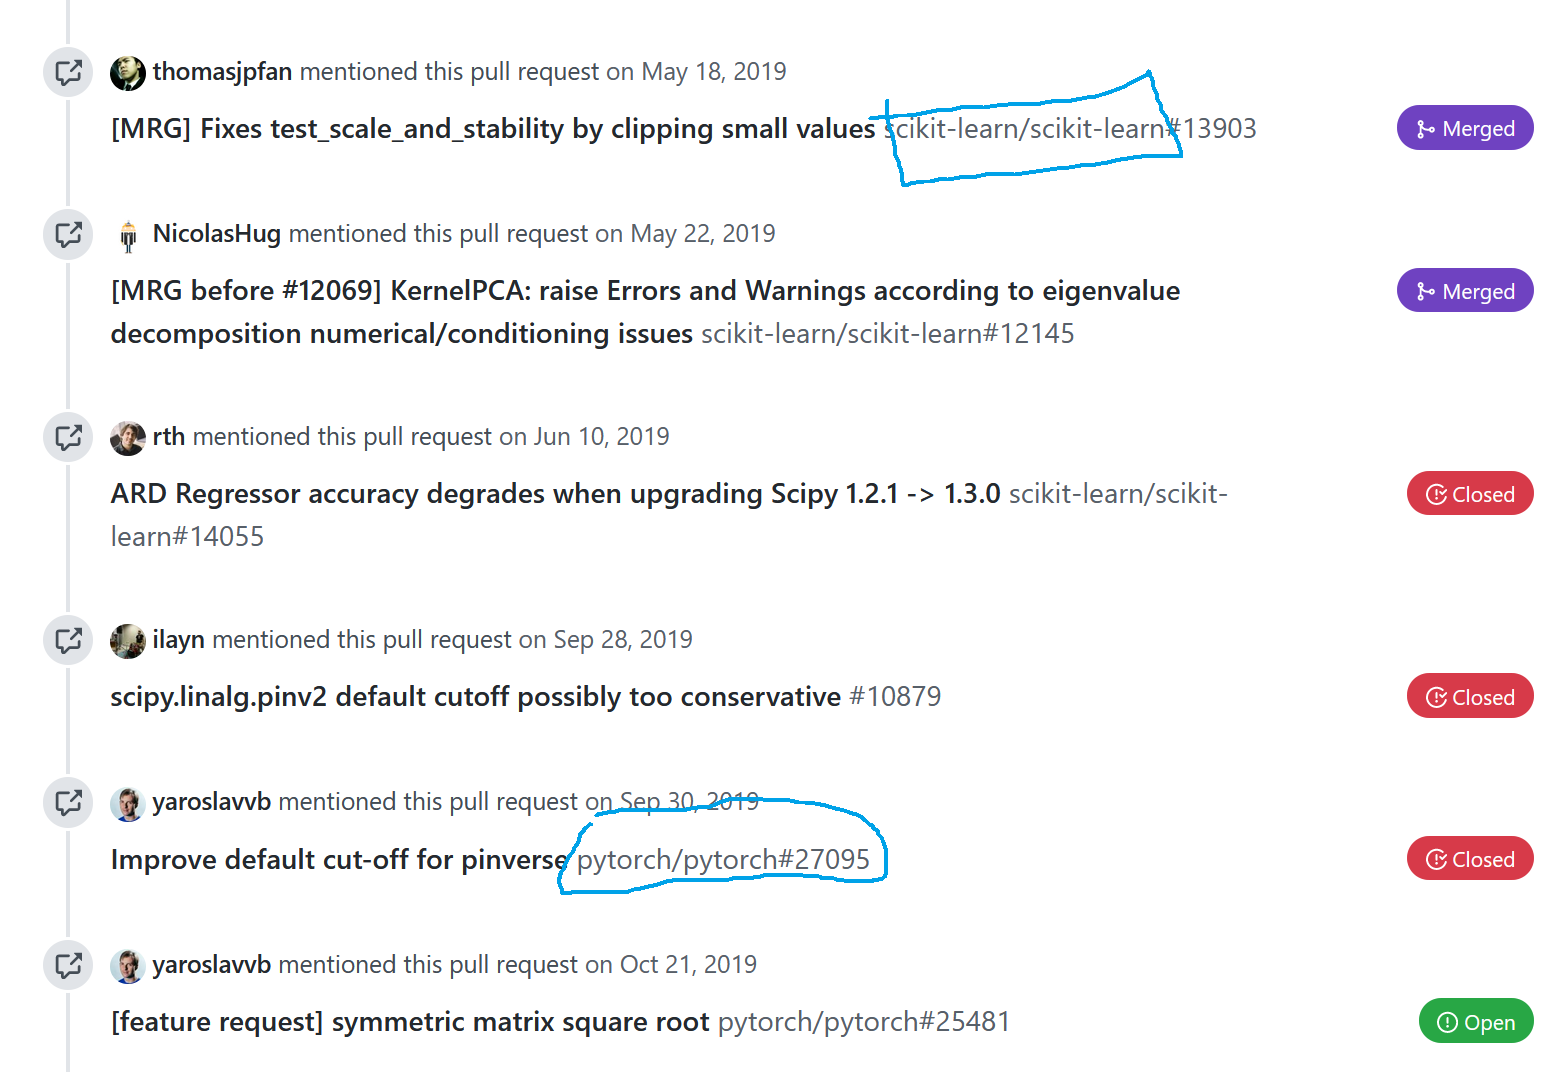
\includegraphics[width=0.5\textwidth]{pinv2}
\par
}
\end{frame}

\begin{frame}{Maintaining SciPy}{Why do it then?}
\begin{itemize}
\item Exceptional teamwork experience
\item High-quality code
\item Professional-grade CI/CD knowledge
\end{itemize}
\end{frame}

\begin{frame}{Thanks}
\begin{description}
\item[social] \begin{tabular}{cl}\faGithubSquare&@ilayn\\\faLinkedinSquare&ilhanpolat\\\faTwitterSquare&\_ilhanpolat\_\\\faEnvelopeSquare&ilhanpolat@gmail.com\end{tabular}
\end{description}
\end{frame}

\end{document}
